\begin{figure}[H]
\centering
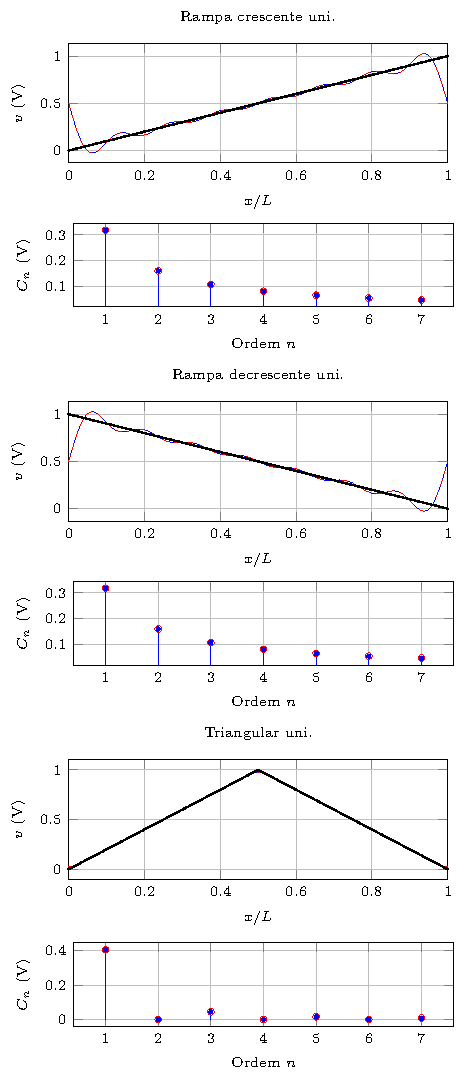
\includegraphics[width=\linewidth,height=0.86\textheight,keepaspectratio]{resultados/figuras/comparacao_basicas_unipolares.pdf}
\caption{Sinais 1 a 3 da Figura 1: ondas unipolares. Para cada sinal, apresentam-se a onda e seu espectro. Preto: amostras; azul: teoria até a ordem 7; vermelho: FFT da simulação.}\label{fig:comparacao1}
\end{figure}
\begin{figure}[H]
\centering
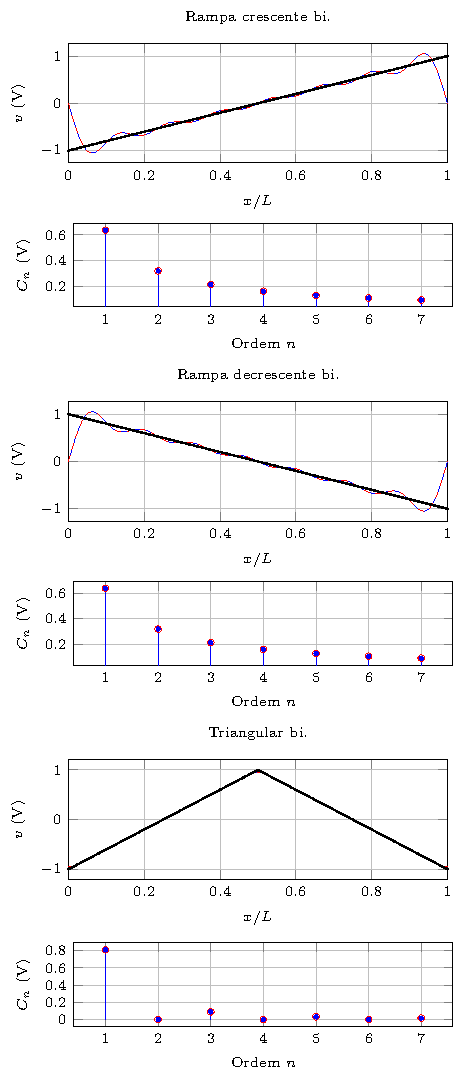
\includegraphics[width=\linewidth,height=0.86\textheight,keepaspectratio]{resultados/figuras/comparacao_basicas_bipolares.pdf}
\caption{Sinais 4 a 6 da Figura 1: ondas bipolares. Para cada sinal, apresentam-se a onda e seu espectro. Preto: amostras; azul: teoria até a ordem 7; vermelho: FFT da simulação.}\label{fig:comparacao2}
\end{figure}
\begin{figure}[H]
\centering
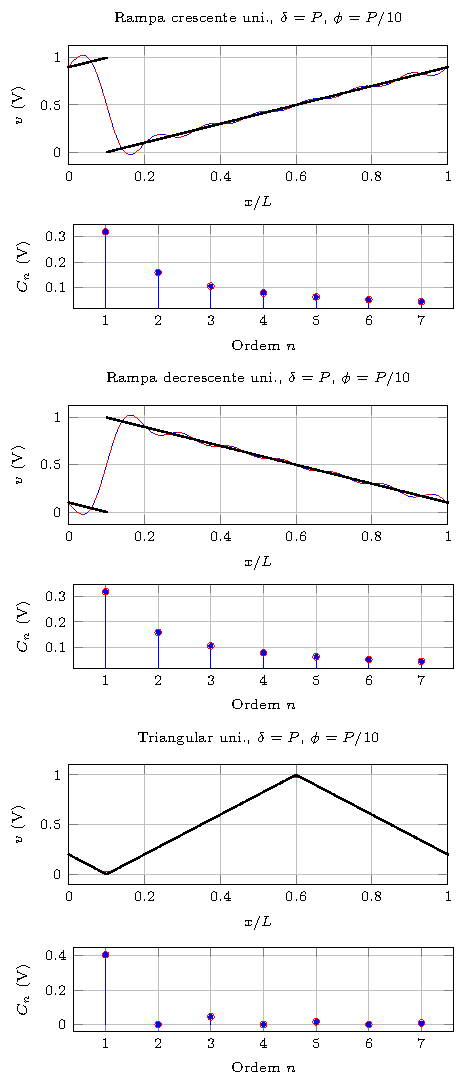
\includegraphics[width=\linewidth,height=0.86\textheight,keepaspectratio]{resultados/figuras/comparacao_deslocadas_P_unipolares.pdf}
\caption{Ondas unipolares deslocadas, $\delta=P$. Para cada sinal, apresentam-se a onda e seu espectro. Preto: amostras; azul: teoria até a ordem 7; vermelho: FFT da simulação.}\label{fig:comparacao3}
\end{figure}
\begin{figure}[H]
\centering
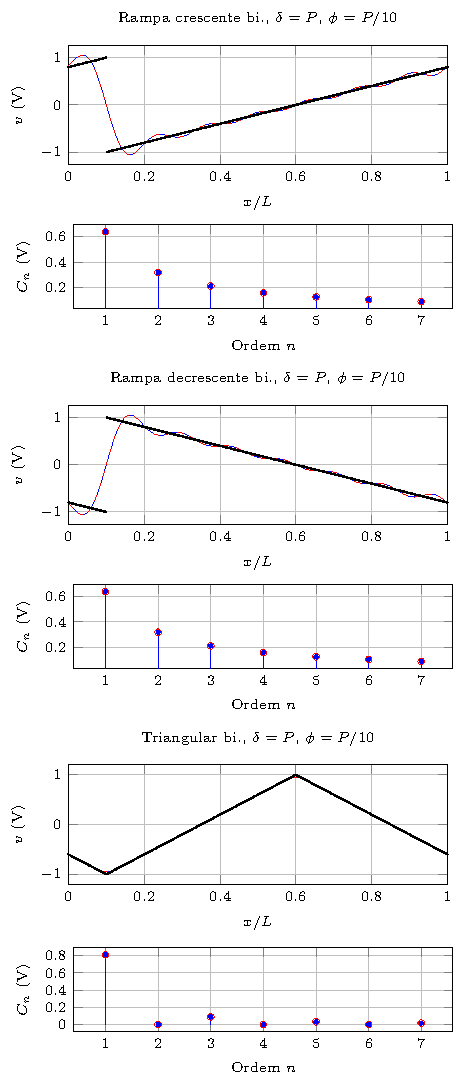
\includegraphics[width=\linewidth,height=0.86\textheight,keepaspectratio]{resultados/figuras/comparacao_deslocadas_P_bipolares.pdf}
\caption{Ondas bipolares deslocadas, $\delta=P$. Para cada sinal, apresentam-se a onda e seu espectro. Preto: amostras; azul: teoria até a ordem 7; vermelho: FFT da simulação.}\label{fig:comparacao4}
\end{figure}
\begin{figure}[H]
\centering
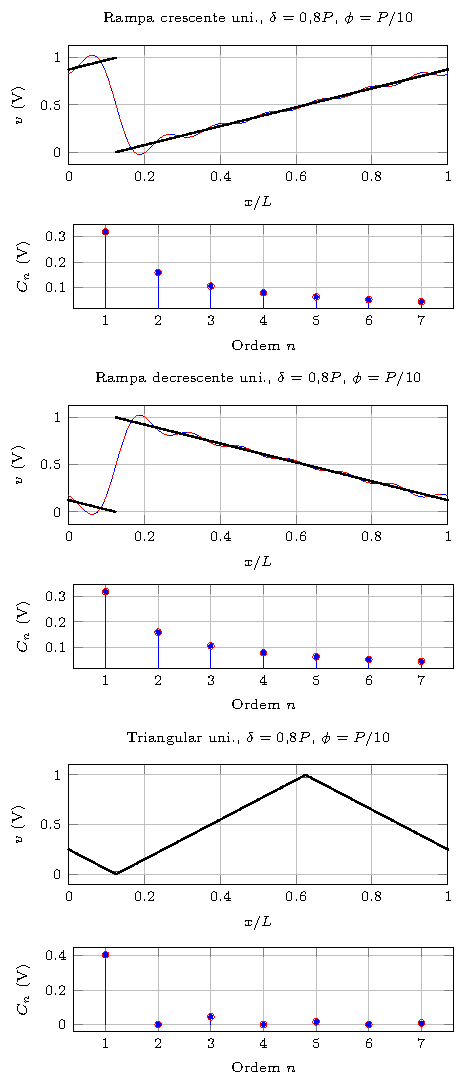
\includegraphics[width=\linewidth,height=0.86\textheight,keepaspectratio]{resultados/figuras/comparacao_deslocadas_08P_unipolares.pdf}
\caption{Ondas unipolares deslocadas, $\delta=0{,}8P$. Para cada sinal, apresentam-se a onda e seu espectro. Preto: amostras; azul: teoria até a ordem 7; vermelho: FFT da simulação.}\label{fig:comparacao5}
\end{figure}
\begin{figure}[H]
\centering
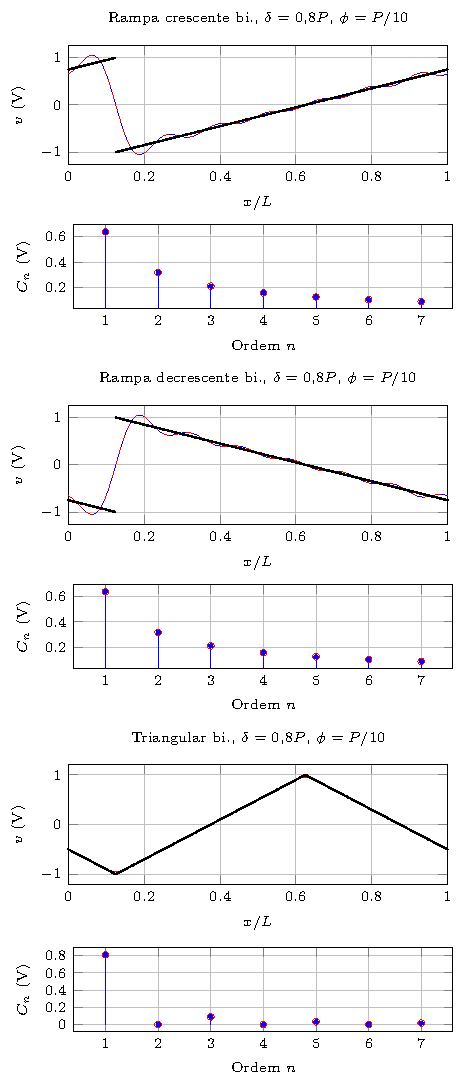
\includegraphics[width=\linewidth,height=0.86\textheight,keepaspectratio]{resultados/figuras/comparacao_deslocadas_08P_bipolares.pdf}
\caption{Ondas bipolares deslocadas, $\delta=0{,}8P$. Para cada sinal, apresentam-se a onda e seu espectro. Preto: amostras; azul: teoria até a ordem 7; vermelho: FFT da simulação.}\label{fig:comparacao6}
\end{figure}
\begin{figure}[H]
\centering
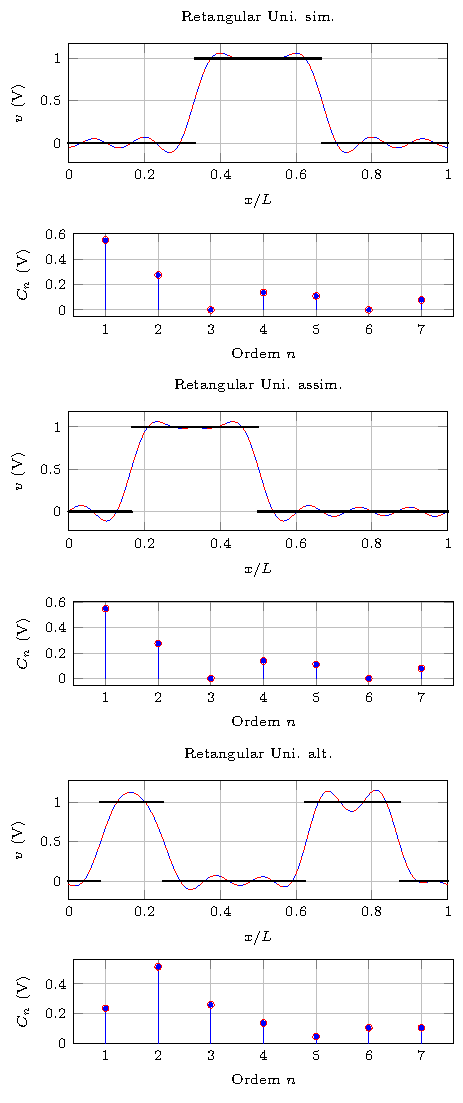
\includegraphics[width=\linewidth,height=0.86\textheight,keepaspectratio]{resultados/figuras/comparacao_retangulares_unipolares.pdf}
\caption{Retangulares unipolares: casos simétrico, assimétrico e alternado. Para cada sinal, apresentam-se a onda e seu espectro. Preto: amostras; azul: teoria até a ordem 7; vermelho: FFT da simulação.}\label{fig:comparacao7}
\end{figure}
\begin{figure}[H]
\centering
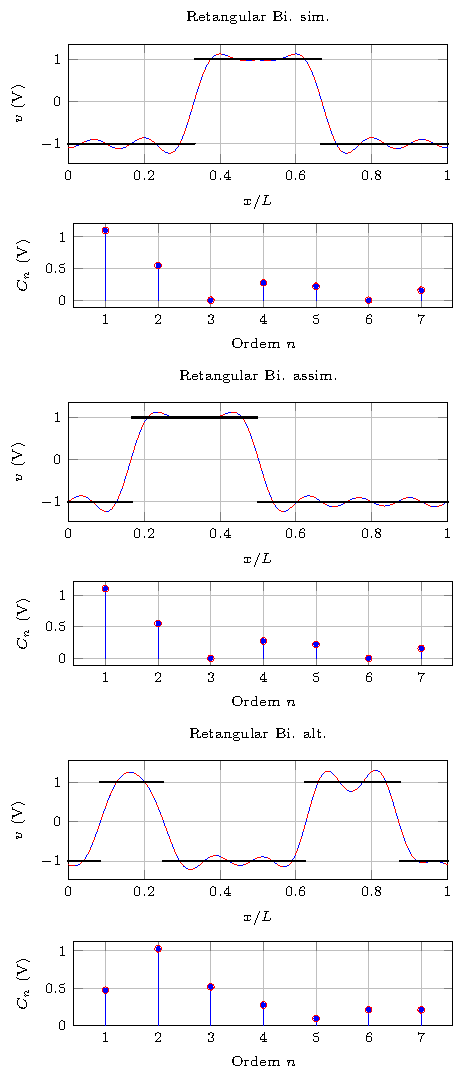
\includegraphics[width=\linewidth,height=0.86\textheight,keepaspectratio]{resultados/figuras/comparacao_retangulares_bipolares.pdf}
\caption{Retangulares bipolares: casos simétrico, assimétrico e alternado. Para cada sinal, apresentam-se a onda e seu espectro. Preto: amostras; azul: teoria até a ordem 7; vermelho: FFT da simulação.}\label{fig:comparacao8}
\end{figure}
